\usetikzlibrary{calc}



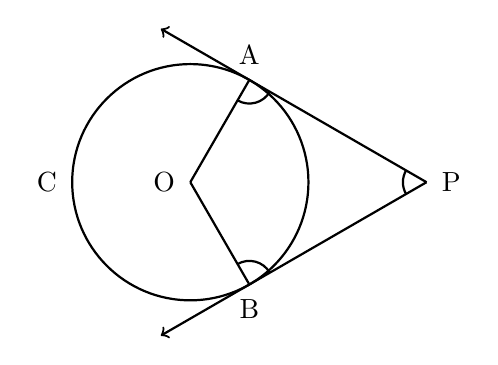
\begin{tikzpicture}[scale=1]

    % Define the center of the circle
    \coordinate (O) at (0,0);

    % Draw the circle
    \draw[thick] (O) circle (1.5);

    % Define points on the circle
    % A and B are positioned so that P forms perfect tangent lines
    \coordinate (A) at (60:1.5);
    \coordinate (B) at (300:1.5);
    \coordinate (C) at (180:1.5);

    % Define the external point P
    % Shifted P slightly to (3,0) to make the lines perfectly tangent to the circle
    \coordinate (P) at (3,0);

    % Draw the lines and segments
    \draw[thick, ->] (P) -- ($(A)!-0.5!(P)$);
    \draw[thick, ->] (P) -- ($(B)!-0.5!(P)$);
    \draw[thick] (O) -- (A);
    \draw[thick] (O) -- (B);

    % Draw the angle arcs
    % Arc at A (trimmed strictly between the radius and tangent line)
    \draw[thick] (A) ++(240:0.3) arc (240:330:0.3);
    % Arc at B (trimmed strictly between the tangent line and radius)
    \draw[thick] (B) ++(30:0.3) arc (30:120:0.3);
    % Arc at P (radius trimmed down to 0.3)
    \draw[thick] (P) ++(150:0.3) arc (150:210:0.3);

    % Add labels for the points
    \node[above, yshift=2pt] at (A) {A};
    \node[below, yshift=-2pt] at (B) {B};
    \node[left, xshift=-2pt] at (C) {C};
    \node[left, xshift=-2pt] at (O) {O};
    \node[right, xshift=2pt] at (P) {P};

\end{tikzpicture}